\documentclass[a4paper, 12pt]{article}

\usepackage{cmap}
\usepackage[hidelinks]{hyperref}
\usepackage[rgb]{xcolor}
\usepackage[warn]{mathtext}
\usepackage{anyfontsize}
\usepackage[T2A]{fontenc}
\usepackage[utf8]{inputenc}
\usepackage[english, russian]{babel}
\usepackage{bm, amssymb,amsfonts,amsmath,cite,enumerate,float,indentfirst}

\usepackage{graphicx}

\usepackage{multirow}
\usepackage{diagbox}

\usepackage{wrapfig}

\usepackage[left=3cm,right=1.5cm,top=2cm,bottom=2cm,bindingoffset=0cm]{geometry}
\usepackage[labelsep=endash]{caption}

\usepackage{setspace}
\setstretch{1.5}
\author{Трунов Владимир Владимирович}
\title{Отчёт о выполнении лабораторной работы 3.3.2 \\ Исследование вольт-амперной характеристики вакуумного диода}
\date{}


\begin{document}
\newpage
	\maketitle
    \newpage
	
	\section{Аннотация}
	В данной работе будет получен удельный элементарный заряд, а также будет экспериментально подтверждён закон трёх вторых.
	
	\section{Теоретическое введение}
	\begin{wrapfigure}{r}{0.3\linewidth} 
		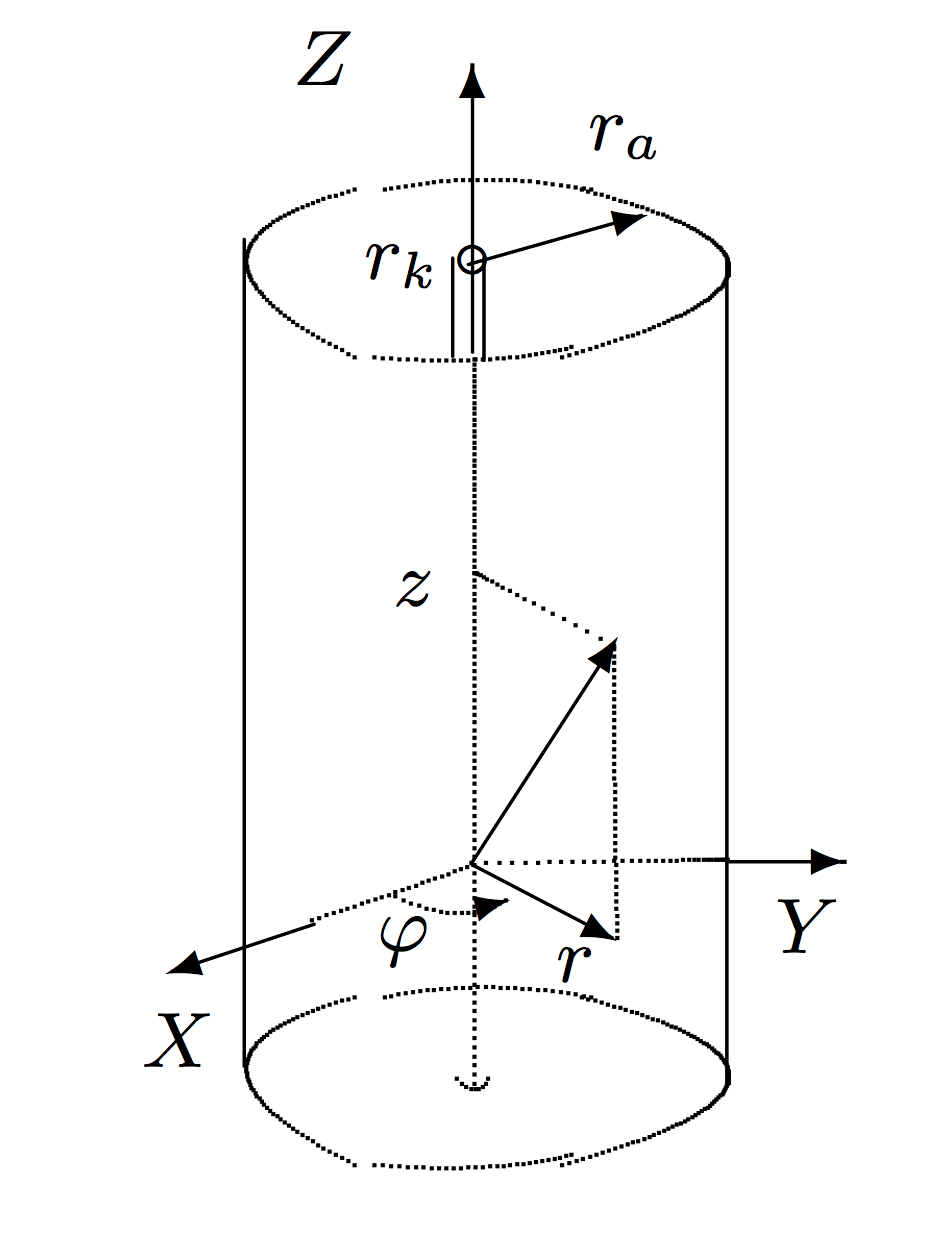
\includegraphics[scale=0.3]{diod}
		\caption{Схема распределения электродов в диоде}
	\end{wrapfigure}
	
	В работе исследуется зависимости прямого тока, проходящего через вакуумный диод, в зависимости от напряжения на нем, а именно та часть вольт-амперной характеристики, в которой электронное облако существенно влияет на распределение электрического поля между катодом и анодом.
	
	Распределение потенциала по радиусу внутри диода определяется уравнением Пуассона в цилиндрических координатах:
	
	\begin{equation}\label{}
		\Delta V = \dfrac{d^2V}{dr^2} + \dfrac{1}{r} + \dfrac{dV}{dr} = - \dfrac{\rho(r)}{\varepsilon_0}
	\end{equation}
	
	При этом плотность заряда $ \rho(r) $ связана с текущим через слой диода толщины $ l $ током $ I $ формулой $ I = -2\pi r \rho(r)v(r)l$. При этом из закона сохранения энергии мы легко находим скорость $ v(r) $ электронов , прошедших через разность потенциалов $ V(r) $: $ \frac{mv^2}{2} = eV(r) $.  Отсюда мы получаем уравнение 
	
	\begin{equation}\label{ur}
	r \dfrac{d^2V}{dr^2} + \dfrac{dV}{dr} = \dfrac{I}{2\pi\varepsilon_0}\sqrt{\dfrac{m}{2eV}}
	\end{equation}
	
	Однако, в дифференциальном уравнении 2-ого порядка относительно $ V(r) $ нам неизвестен ток I, зависящий от V. Для доопределения уравнения будем полагать:
	
	\begin{equation}\label{usl}
	\dfrac{dV}{dt}\bigg |_{r=r_k} = 0
	\end{equation} 
	
	Наше предположение означает что вблизи катода пространственный заряд электронов полностью экранирует поле анодной разности потенциалов.
	
	Уравнение \eqref{ur} является нелинейным. Попробуем  найти некое частное решение, где $ V_a = V_{a0}, $ при котором ток $ I = I_0 $. Тогда выражения 
	
	\begin{equation}\label{}
	I = I_0 \left( \dfrac{V_a}{V_{a0}} \right) ^{3/2}, \qquad V(r) = V_{a0}(r)\dfrac{V_a}{V_{a0}}
	\end{equation}
	
	являются решением уравнения \eqref{ur}, что проверяется подстановкой. В общем виде решение записывается в виде
	
	\begin{equation}\label{3/2}
	I = \dfrac{8\sqrt{2}\pi \varepsilon_0 l}{9}\sqrt{\dfrac{e}{m}}\dfrac{1}{r_a\beta^2} V^{3/2}
	\end{equation}
	
	Это и есть так называемый "<закон трех вторых"> -- ток в вакуумном диоде пропорционален напряжению на нем в степени 3/2. Он справедлив при любой геометрии электродов, если ток не слишком велик (т.е. пока выполнено условие \eqref{usl}). 
	
	Так как нам нужно найти удельный заряд электрона, выпишем в явном виде его из уравнения \eqref{3/2}:
	
	\begin{equation}\label{e/m}
	 	\frac{e}{m} = \frac{81 r^2_a \beta ^ 4}{128 \pi ^2 \varepsilon_0 l^2} \cdot \frac{I^2}{V^3} = k \frac{I^2}{V^3}
	\end{equation}
	
	Таким образом, удельный заряд электрона определяется из отношения квадрата тока к кубу напряжения, умноженный на коэффициент, зависящий от параметров установки.
	
	\section{Экспериментальная установка}
	\begin{figure}[H]
		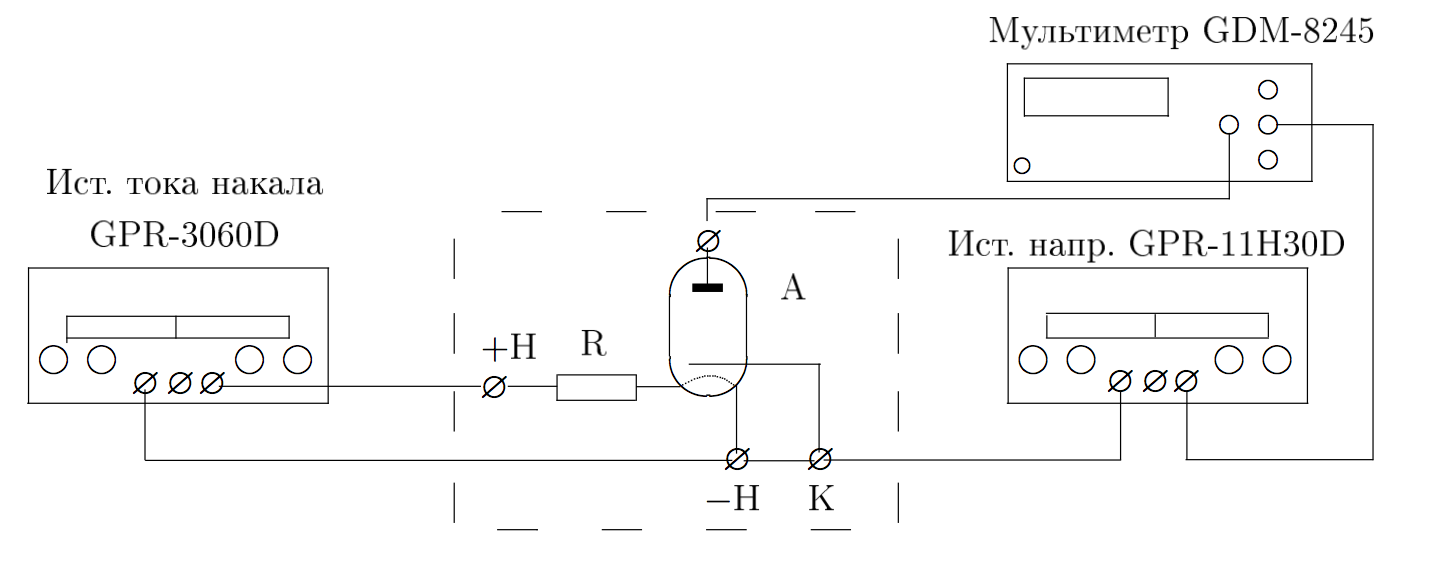
\includegraphics[width=15cm]{lab}
		\caption{Схема экспериментальной установки}
	\end{figure}
	
	В работе используется диод 2Ц2С с косвенным накалом. Радиус его катода $ r_k = 0,9 $ мм, радиус анода $ r_a = 9,5  $ мм, коэффициент $ \beta^2 = 0,98 $, длина слоя центральной части катода, покрытой оксидным слоем $ l = 9 $ мм.
	
	Для подогрева катода и анода используются стабилизированные источники постоянного тока и напряжения. В цепь накала включено предохранительное напряжение $ R $. Анодное напряжение измеряется вольтметром источника питания, анодный ток --- многопредельным мультиметром GDM-8245. 
	
	
	\section{Ход работы}
	
	Сперва, вычислим коэффициент $ k $:
	
	\begin{equation}\label{}
		k = \frac{81 \cdot (9,5 \cdot 10 ^ {-3}) ^ 2 \cdot 0,98 ^ 4}{62 \cdot 2 \cdot 3, 14 ^ 2 \cdot (8,85 \cdot 10 ^ {-12}) ^ 2 \cdot (9 \cdot 10 ^ {-3})^2} \approx 8,4 \cdot 10 ^ {20}
	\end{equation}
	
	Установим ток накала на $ I_н = 1,3 $ А, а начальное анодное напряжение на $ V = 0.5  $ В.  Проведем измерения анодного тока в зависимости от напряжения, изменяя его от $ 0,5 $ до 50 В. 
	
	Затем проведем аналогичные измерения для других токов накала: $ 1,4 \; А; 1,5 \; А; 1,6 $ А. Результаты занесем в таблицу \ref{res}.
	
	\begin{table}[H]
		\centering
		\begin{tabular}{|l|l|l|l|l|}
			\hline
			\multirow{2}{*}{$V,$ В} & $I_a = 1,3$ А & $I_a = 1,4$ А & $I_a = 1,5$ А & $I_a = 1,59$ А  \\ \cline{2-5}
			& $I$, мкА & $I$, мкА & $I$, мкА & $I$, мкА \\ \hline \hline
		0,5 & 4,29  & 7,75  & 15,75  & 23,8  \\ \hline
        1.0 & 13,08  & 19,8  & 28,05  & 39,5  \\ \hline
        1,5 & 26,01  & 33,7  & 45,8  & 58,25  \\ \hline
        2,0 & 40  & 48,5  & 62,15  & 79,2  \\ \hline
        2,5 & 56,3  & 66,3  & 84,5  & 103  \\ \hline
        3,0 & 74,5  & 89,9  & 103  & 123,8  \\ \hline
        3,5 & 94  & 109,8  & 128,7  & 152,6  \\ \hline
        4,0 & 116,2  & 133  & 152,3  & 176,55  \\ \hline
        4,5 & 138,7  & 154,8  & 178,5  & 203,8  \\ \hline
        5,0 & 162,4  & 183,1  & 203,8  & 229  \\ \hline
        5,5 & 191,3  & 209,3  & 231,7  & 259,1  \\ \hline
        6,0 & 216,5  & 235,6  & 259,2  & 288,5  \\ \hline
        7,0 & 270,6  & 295,3  & 323,6  & 356  \\ \hline
        8,0 & 331,8  & 360,3  & 390,1  & 424,7  \\ \hline
        9,0 & 399,3  & 431,3  & 495  & 501,2  \\ \hline
        10,0 & 472  & 499,2  & 571  & 619  \\ \hline
        15,0 & 914  & 957  & 1006  & 1070  \\ \hline
        20,0 & 1417  & 1493,6  & 1554  & 1623  \\ \hline
        25,0 & 2002  & 2094,5  & 2175  & 2256  \\ \hline
        30,0 & 2639  & 2764  & 2848  & 2940  \\ \hline
        35,0 & 3314  & 3473  & 3571  & 3669  \\ \hline
        40,0 & 4028  & 4243  & 4358  & 4465  \\ \hline
        45,0 &4782  & 5137  & 5257  & 5392  \\ \hline
        50,0 & 5636  & 6003  & 6151  & 6282  \\ \hline
		\end{tabular}
		\caption{Результаты измерений}
		\label{res}
	\end{table}
	Построи график (рис. \ref{граф}) зависимости в двойном логарифмическом масштабе и убедися, что на зависимость почти полносью соответствует линейной.
    
    \begin{figure}[H]
		\centering
		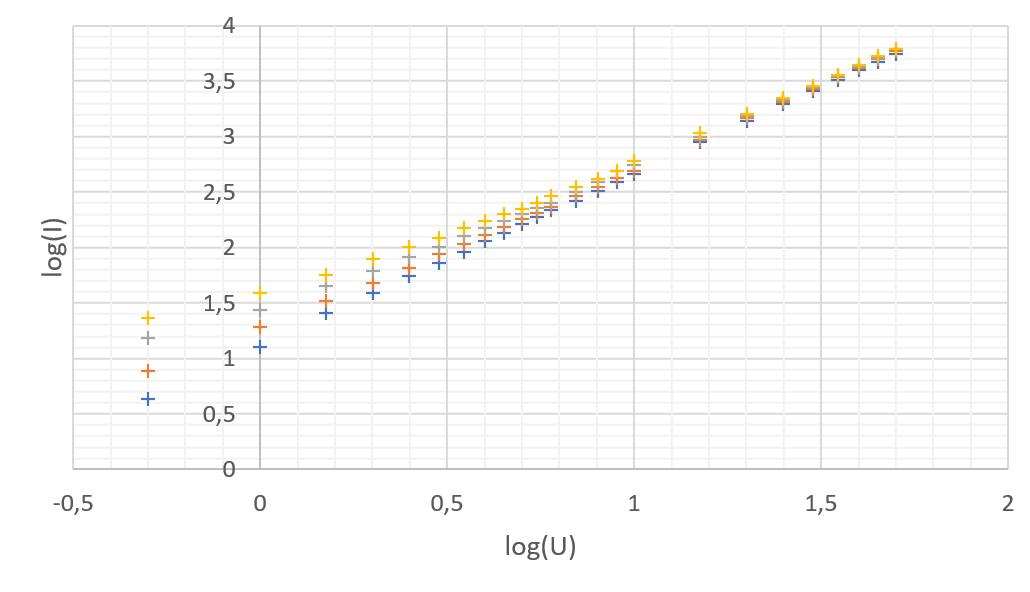
\includegraphics[scale=0.4]{log.png}
		\caption{Графики зависимости силы тока накала от напряжения}
		\label{граф}
	\end{figure}
    
    
	Построим график (рис. \ref{граф}) зависимости $I_a$ от $V_a$. 
	
	\begin{figure}[H]
		\centering
		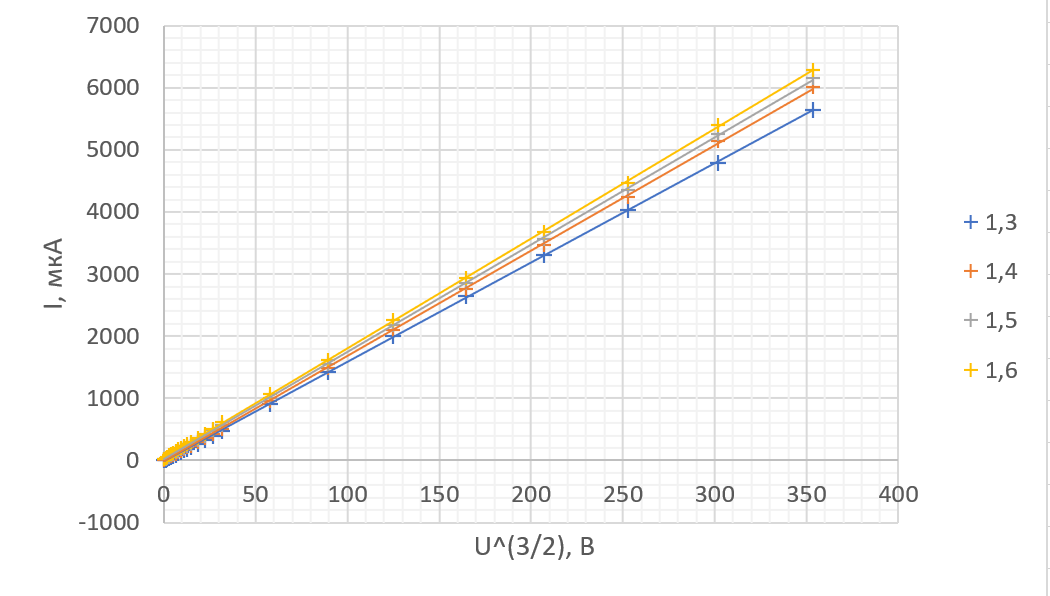
\includegraphics[scale=0.7]{graph_3_2.png}
		\caption{Графики зависимости силы тока накала от напряжения}
		\label{граф}
	\end{figure}
	
	Определив коэффициент наклона $a = \dfrac{\frac{e}{m}}{k}$, найдём удельный заряд для каждого тока. В мы получаем:
	
	\begin{table}[!ht]
    \centering
    \begin{tabular}{|1|l|l|l|l|}
    \hline
        $I_н$, A & 1,3  & 1,4 & 1,5 & 1,6 \\ \hline
       $a$ & 15,97 & 16,94 & 17,30 & 17,67 \\ \hline
       $\sigma$ & 0,03   & 0,03   & 0,02  &   0,03 \\ \hline
    \end{tabular}
\end{table}

\begin{table}[!ht]
    \centering
    \begin{tabular}{|l|l|l|l|1|}
    \hline
        $I_н$, A & 1,3 & 1,4 & 1,5 & 1,6\\ \hline
        $\dfrac{e}{m}, 10^{11} \frac{Кл}{кг}$  & 2,14 & 2,41 & 2,51 & 2,62 \\ \hline
        $\sigma, 10^{11} \frac{Кл}{кг}$ & 0,02 & 0,02 & 0,02 & 0,02 \\ \hline
    \end{tabular}
\end{table}

	\section{Вывод}
	Ни одно из значений удельного заряда не совпало с табличным $\frac{e}{m} = 1,759 \cdot 10^{11}$ Кл/кг. Ближе всего оказалось значение для тока накала  $I_н = 1,3$ А; это можно связать с тем, что вокруг катода сосредоточено мало зарядов, что соответствует условию \eqref{usl}. Точность измерений значительно уменьшилась из-за того, что катод просто не успевал полносью прогреться за выделенное время, поэтому показания приборов постоянно менялись. В целом все характерные зависимости были экспериментально подтверждены.
	
\end{document}